\section{Halvledardioden}
\textbf{HAREC a.\ref{HAREC.a.2.5}\label{myHAREC.a.2.5}}
\index{halvledardiod}
\index{diod}
\index{diod!halvledardiod}

\subsection{Allmänt}
I en strömkrets kan av olika anledningar ström tillåtas att flyta i en riktning
men kanske inte i den motsatta. En anordning med en sådan funktion kallas för
en diod.

Först bestod en diod av två elektroder i vakuum (se avsnitt
\ref{vakuumdioden}). Därav namnet vakuumdiod.
Numera består en diod oftast av någon halvledare. Därav namnet halvledardiod.

\begin{figure}
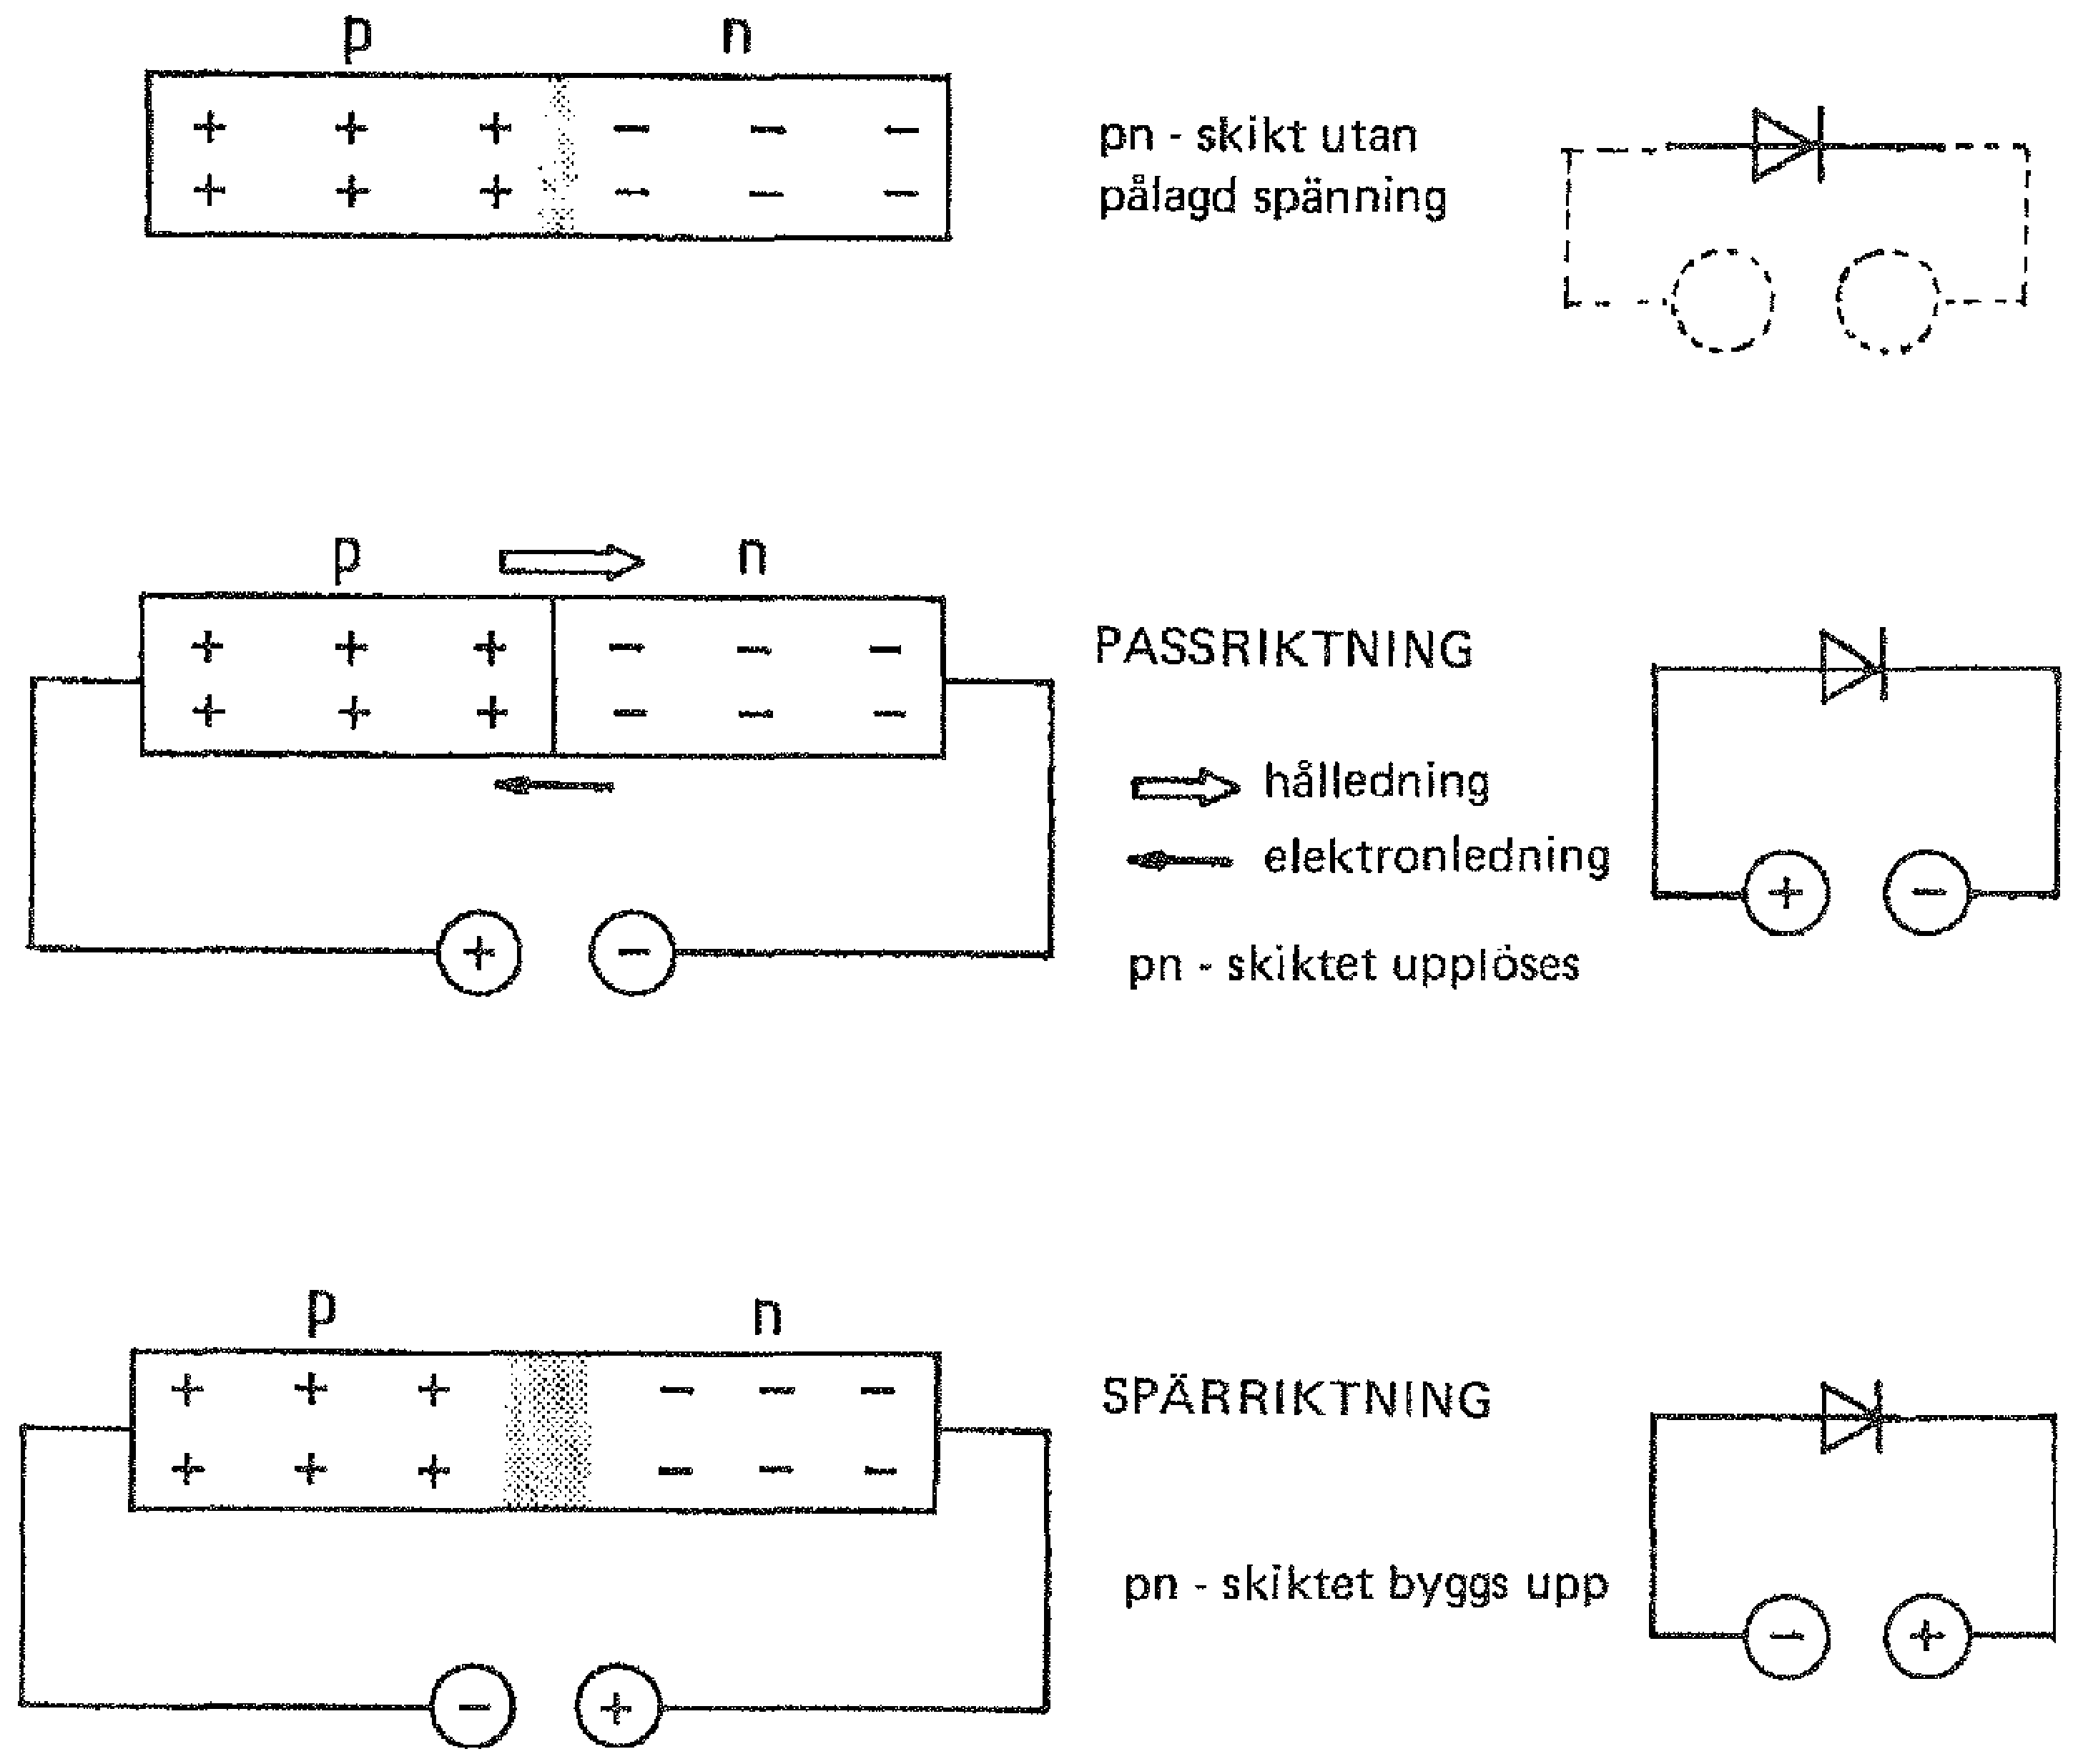
\includegraphics[width=\textwidth]{images/cropped_pdfs/bild_2_2-12.pdf}
\caption{Spärrskiktet i en halvledardiod}
\label{fig:BildII2-12}
\end{figure}

Bild \ref{fig:BildII2-12} överst illustrerar en halvledardiod bestående av ett
P-ledande och ett N-ledande materialskikt som fogats samman.

Mellan de båda skikten utbildas ett tunt gränsskikt som inte innehåller
laddningsbärare. Detta skikt kan vara ledande eller icke ledande -- ett
spärrskikt -- beroende på polariseringen.

\subsection{Halvledardiodens karaktär}
\textbf{HAREC a.\ref{HAREC.a.2.5.1.2}\label{myHAREC.a.2.5.1.2}}

\subsubsection{Diod i framriktningen}
\index{diod!framriktning}
\index{diod!framström}
\index{diod!framspänningsfallet}

Förbinder man den positiva polen på en spänningskälla med P-skiktet i en diod
och den negativa polen med N-skiktet så är dioden polariserad i
\emph{framriktningen}, detta illustreras i bild \ref{fig:BildII2-12} mitten.
Spärrskiktet upplöses då och en \emph{framström}
(eng. \emph{forward current}) flyter genom dioden.
Elektronerna flyter till den positiva polen och hålen till den negativa polen.
Över anslutningarna ligger en spänning, \emph{framspänningsfallet}
(eng. \emph{forward voltage}), som varierar med strömmen och temperaturen.
Spänningsfallet och strömmen ger på normalt sett diodens \emph{förlusteffekt}.

\subsubsection{Diod i backriktningen}
\index{diod!spärriktningen}
\index{diod!backriktningen}
\index{diod!zenereffekt}

\emph{Backspänning, backström, läckström, spärriktning}

Förbinder man i stället den negativa polen på en spänningskälla med P-skiktet i
en diod och den positiva polen med N-skiktet så är dioden polariserad i
\emph{spärriktningen} eller \emph{backriktningen}, så som illustreras i
bild \ref{fig:BildII2-12} underst.
Spärrskiktet blir då ännu kraftigare.

Endast en obetydlig ström \(I_{SP}\) flyter genom dioden i spärriktningen, även vid 
ökande spänning \(U_{SP}\).
Men över en viss spänning ökar strömmen snabbt -- den så kallade zenereffekten
uppstår.
Dioden kan då lätt förstöras av en alltför hög ström.

\subsubsection{Diod i strömkrets}
\index{diod!inkoppling}
\index{diod!anod}
\index{diod!katod}
\index{diod!PANK}

När en diod kopplas in i en strömkrets är det nödvändigt att dioden vänds så att
ström kan flyta igenom den i önskad riktning.

Anslutningen till en diods P-skikt kallas för \emph{anod} och kopplas normalt
mot strömkretsens positiva pol.

Motsvarande anslutning från N-skiktet på en diod kallas \emph{katod} och kopplas
normalt mot strömkretsens negativa pol.

För att komma ihåg hur en diod ska vändas så används anod och katod i en
minnesregel som lyder Positiv~Anod~Negativ~Katod vilket förkortas \textbf{PANK}.

En diods katod märks ut med ett streck på eller en markering i höljet som ska
motsvara strecket framför pilen i diodens schemasymbol.

\subsubsection{Diodens ström-spänningsförhållande}

\begin{figure}
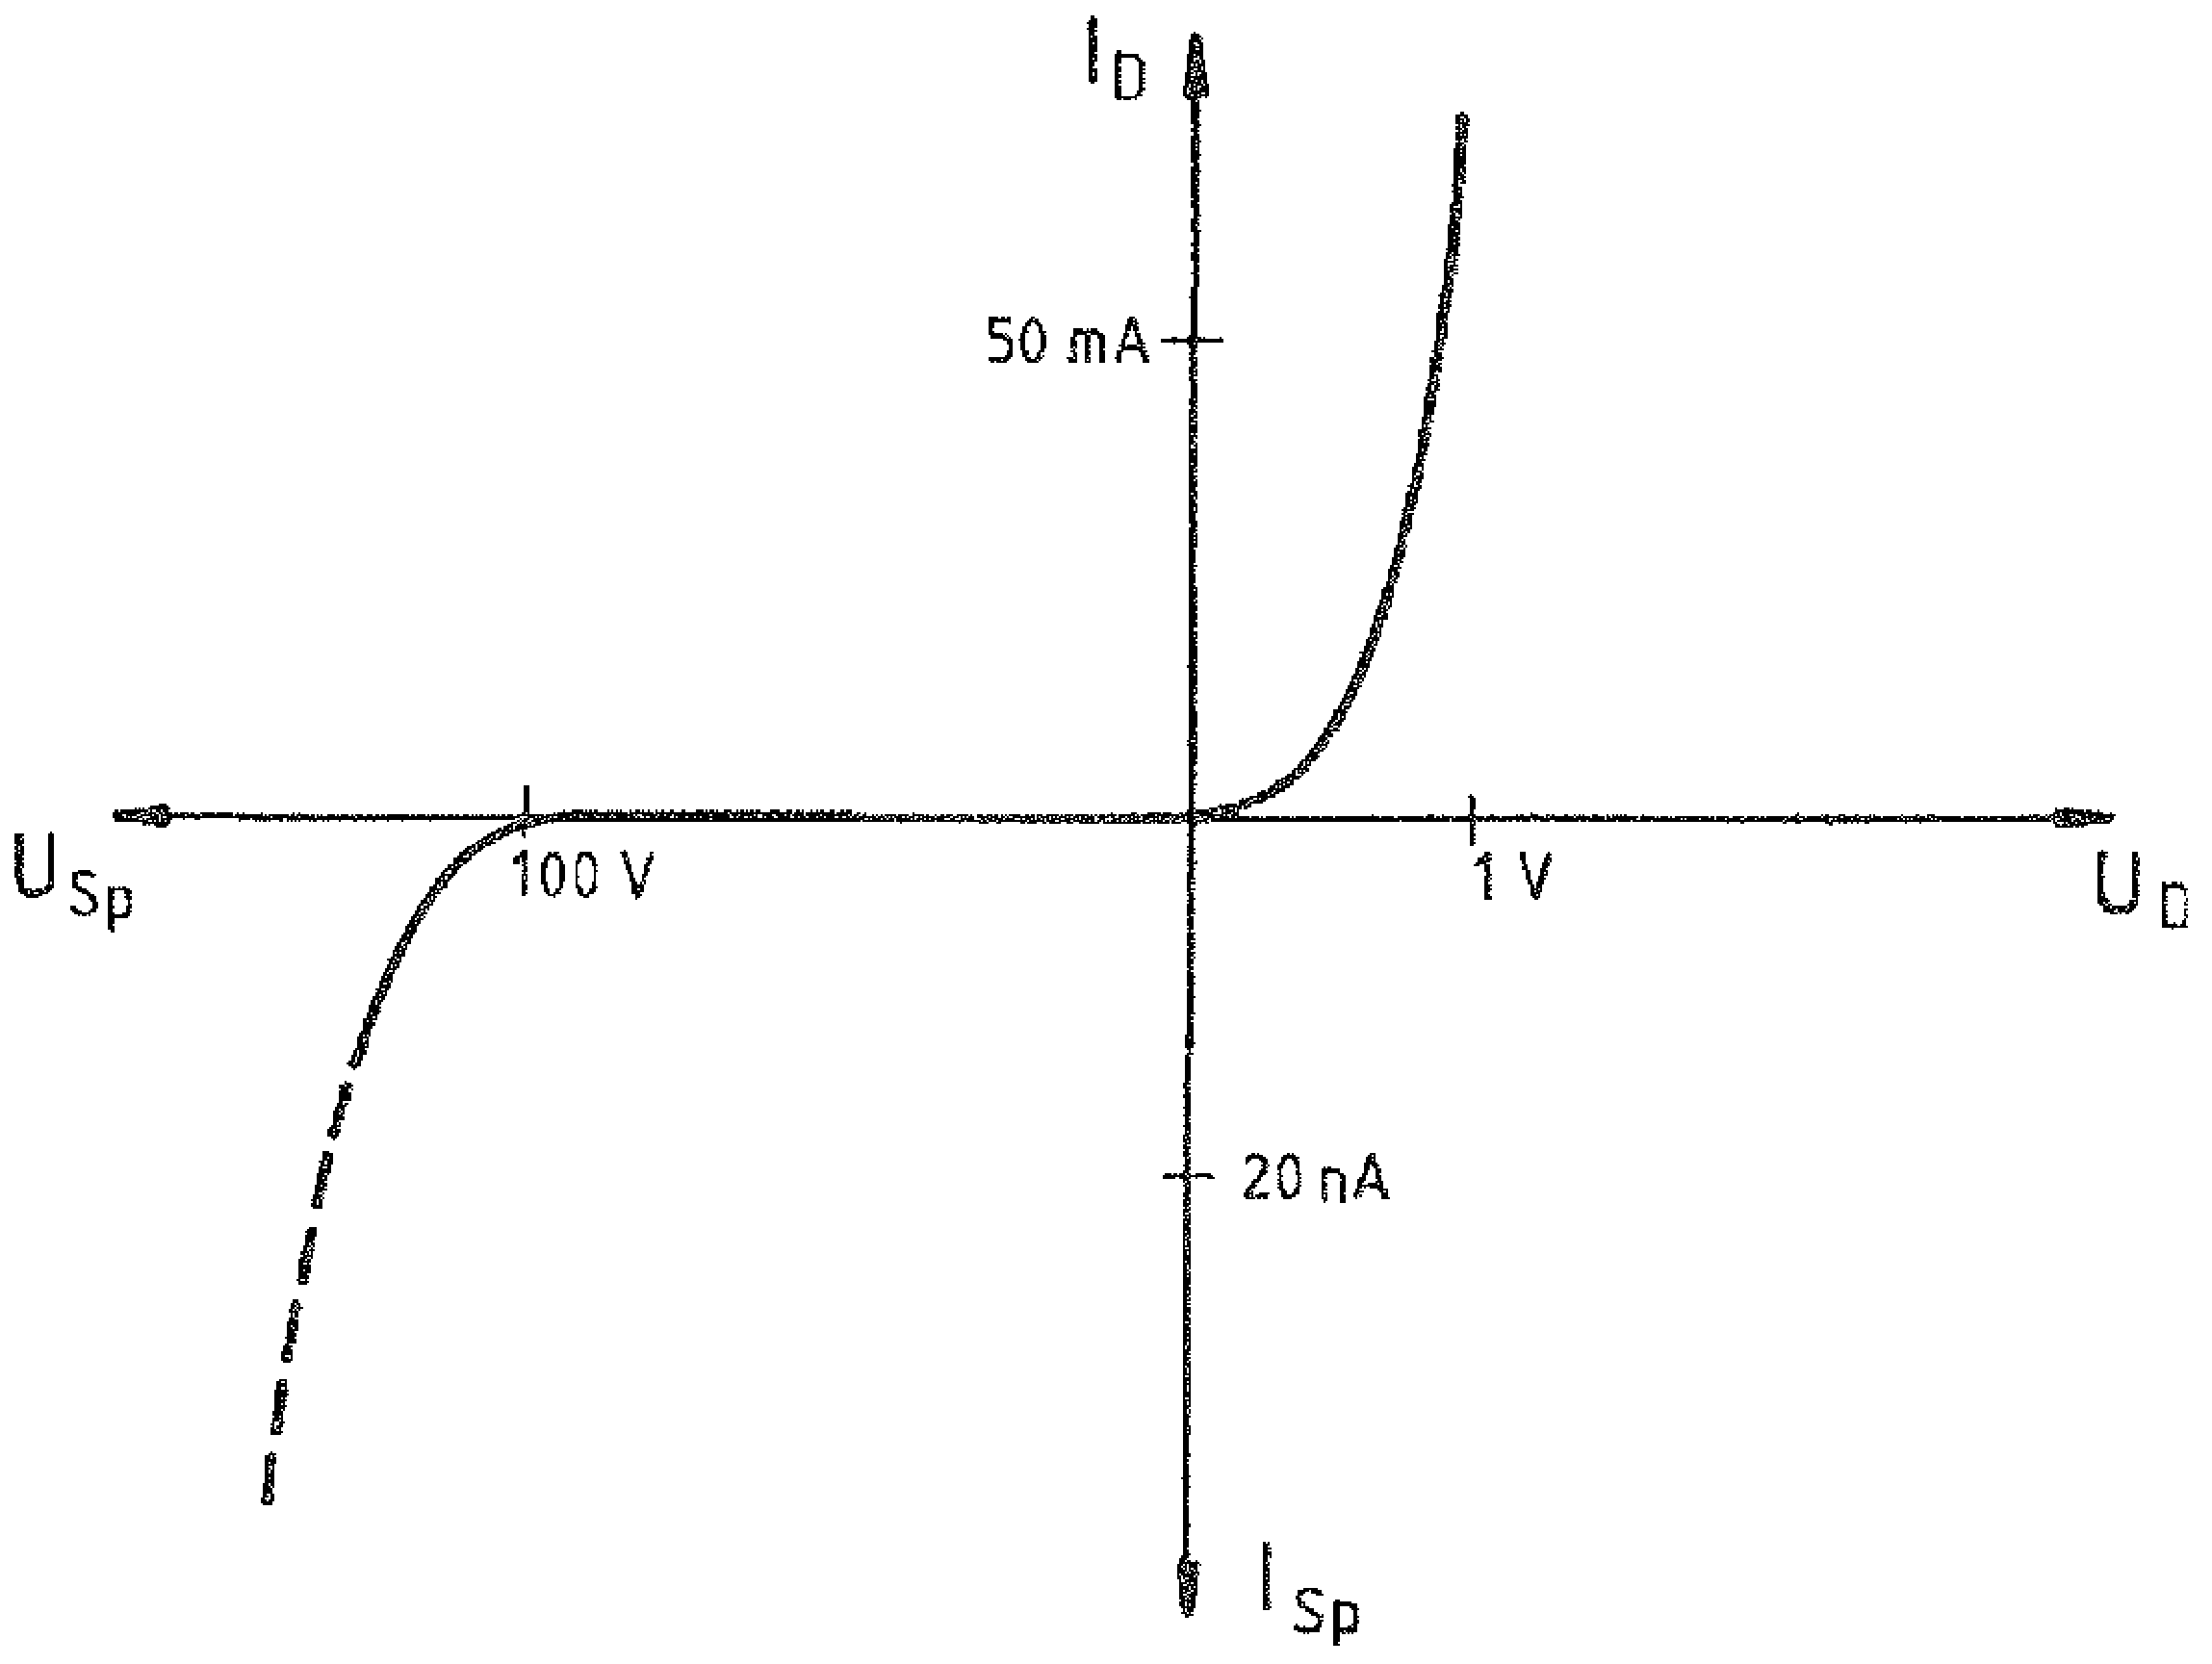
\includegraphics[width=\textwidth]{images/cropped_pdfs/bild_2_2-13.pdf}
\caption{Halvledardiodens karaktäristik}
\label{fig:BildII2-13}
\end{figure}

Bild \ref{fig:BildII2-13} visar en diods ström-spänningsförhållande.

Strömmen \(I_D\) börjar att flyta när spänningen \(U_D\) har nått ett
tröskelvärde (vid kiseldioder 0,6~V).
När spänningen ökar ytterligare däröver, ökar även strömmen.

Produkten av spänningsfallet över dioden och strömmen genom den kallas
förlusteffekt. Denna värmer upp dioden. Vid för hög temperatur förstörs
kristallstrukturen. En kiselkristall kan klara upp till 200~\degree C medan en
germaniumkristall bara klarar 75~\degree C.

\subsection{Diodtillämpningar}
\textbf{HAREC a.\ref{HAREC.a.2.5.1.1}\label{myHAREC.a.2.5.1.1}}

Bild \ref{fig:BildII2-14} illustrerar flera olika schemasymboler för
dioder.

\begin{wrapfigure}[13]{R}{0.5\textwidth}
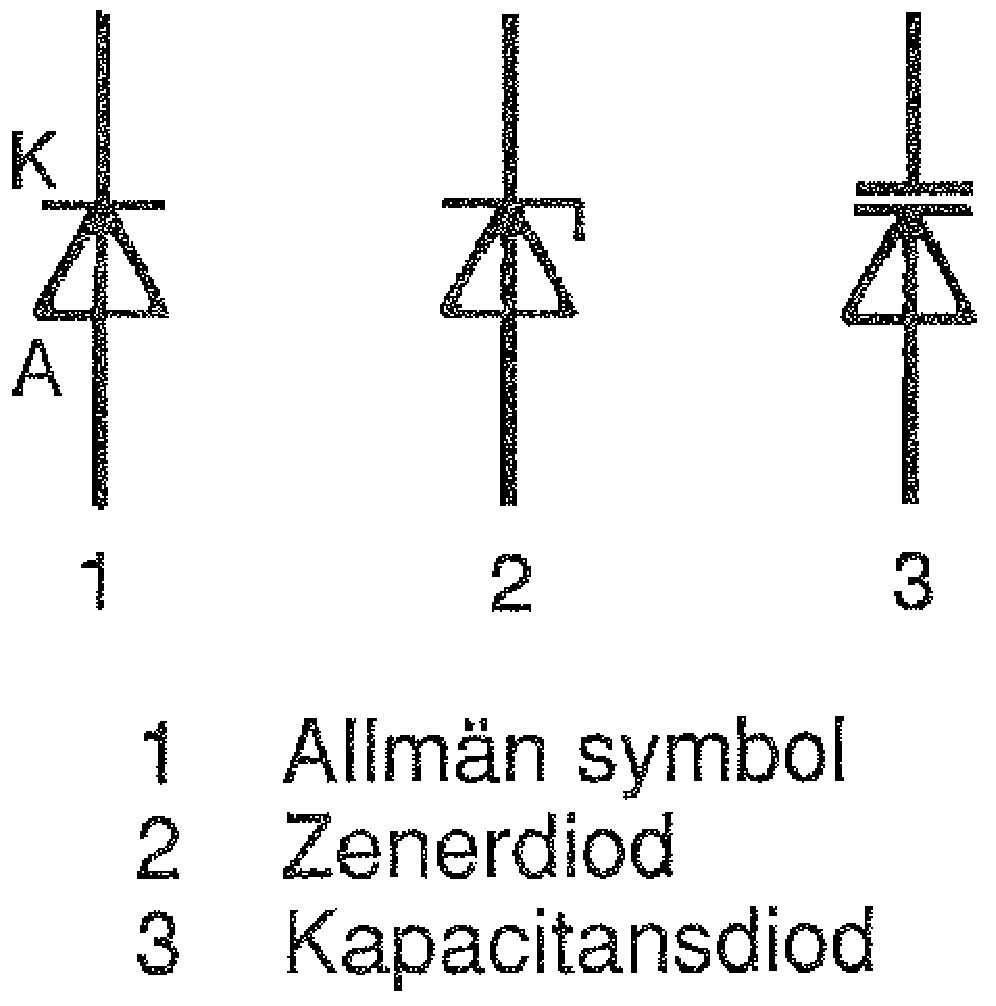
\includegraphics[width=0.5\textwidth]{images/cropped_pdfs/bild_2_2-14.pdf}
\caption{Schemasymboler för dioder}
\label{fig:BildII2-14}
\end{wrapfigure}

Likriktning är den vanligaste tillämpningen för dioder (se kapitel \ref{kraftaggregat}).
Halvledardioder utförs även för en rad andra ändamål och finns i en mängd
varianter.

\subsubsection{Dioder för spänningsstabilisering (zenerdiod).}
\index{zenerdiod}
\index{diod!zener}

  Inom ett visst område är spänningsfallet över en zenerdiod i en strömkrets
  i det närmaste konstant medan strömmen varierar. Denna egenskap kallas
  zenereffekt och används för konstanthållning av spänning.

  Det finns zenerdioder för många olika spänningar och effekter.

\subsubsection{Dioder som variabla kondensatorer (kapacitansdiod, VariCap)}
\label{varicap}
\index{varicap}
\index{diod!varicap}

  När en diod är polariserad i spärriktningen bildas ett spärrskikt.
  Olika polariseringsspänning alstrar olika tjocka spärrskikt och en spärrad diod
  har på så sätt egenskaper som liknar dem i en variabel kondensator. Det finns
  dioder där reglerbarheten av kapacitansen är speciellt utvecklad.

\subsubsection{Lysdioder (LED)}
\index{lysdiod}
\index{diod!lysdiod}
\index{LED}
\index{diod!LED}
\index{laserdiod}
\index{diod!laserdiod}

\emph{Lysdiod} (eng. \emph{Light Emitting Diode (LED)}) är en diod anpassad för
att leverera ljus, ofta synligt sådant.
Lysdioder finns tillgängliga med infrarött, rött, orange, gult, grönt,
blått och vitt ljus.
En variant av lysdiod är laserdioden, som bland annat används för överföring
över optisk fiber.

När en diod är polariserad i passriktningen frigörs energi i spärrzonen.
Det sker genom rekombination av par av laddningsbärare, varvid det normalt avgår
energi i form av värme.
Vid en viss inblandning av främmande atomer avgår istället ljus.

Spänningfallet över en lysdiod är ungefär dubbelt så stort som över en
kiseldiod, det vill säga ungefär 1,5~volt.
Det normala spänningsfallet bör alltid kontrolleras för korrekt dimensionering
av kretsen.
Ljusstyrkan är proportionell mot strömmen, som normalt har värden mellan 10 och 50~mA.
En lysdiod bör ha ett strömbegränsande motstånd i serie för att strömmen
inte ska bli för stor och lysdioden åldras i förtid eller rent av gå sönder.

Moderna högeffektslysdioder kräver en konstantströmsmatning och kan ha betydligt
högre spänning.
Dessa har blivit tillgängliga till lågt pris och populära för experiment.

\subsection{Vakuumdioden i jämförelse med halvledardioden}

\begin{figure}
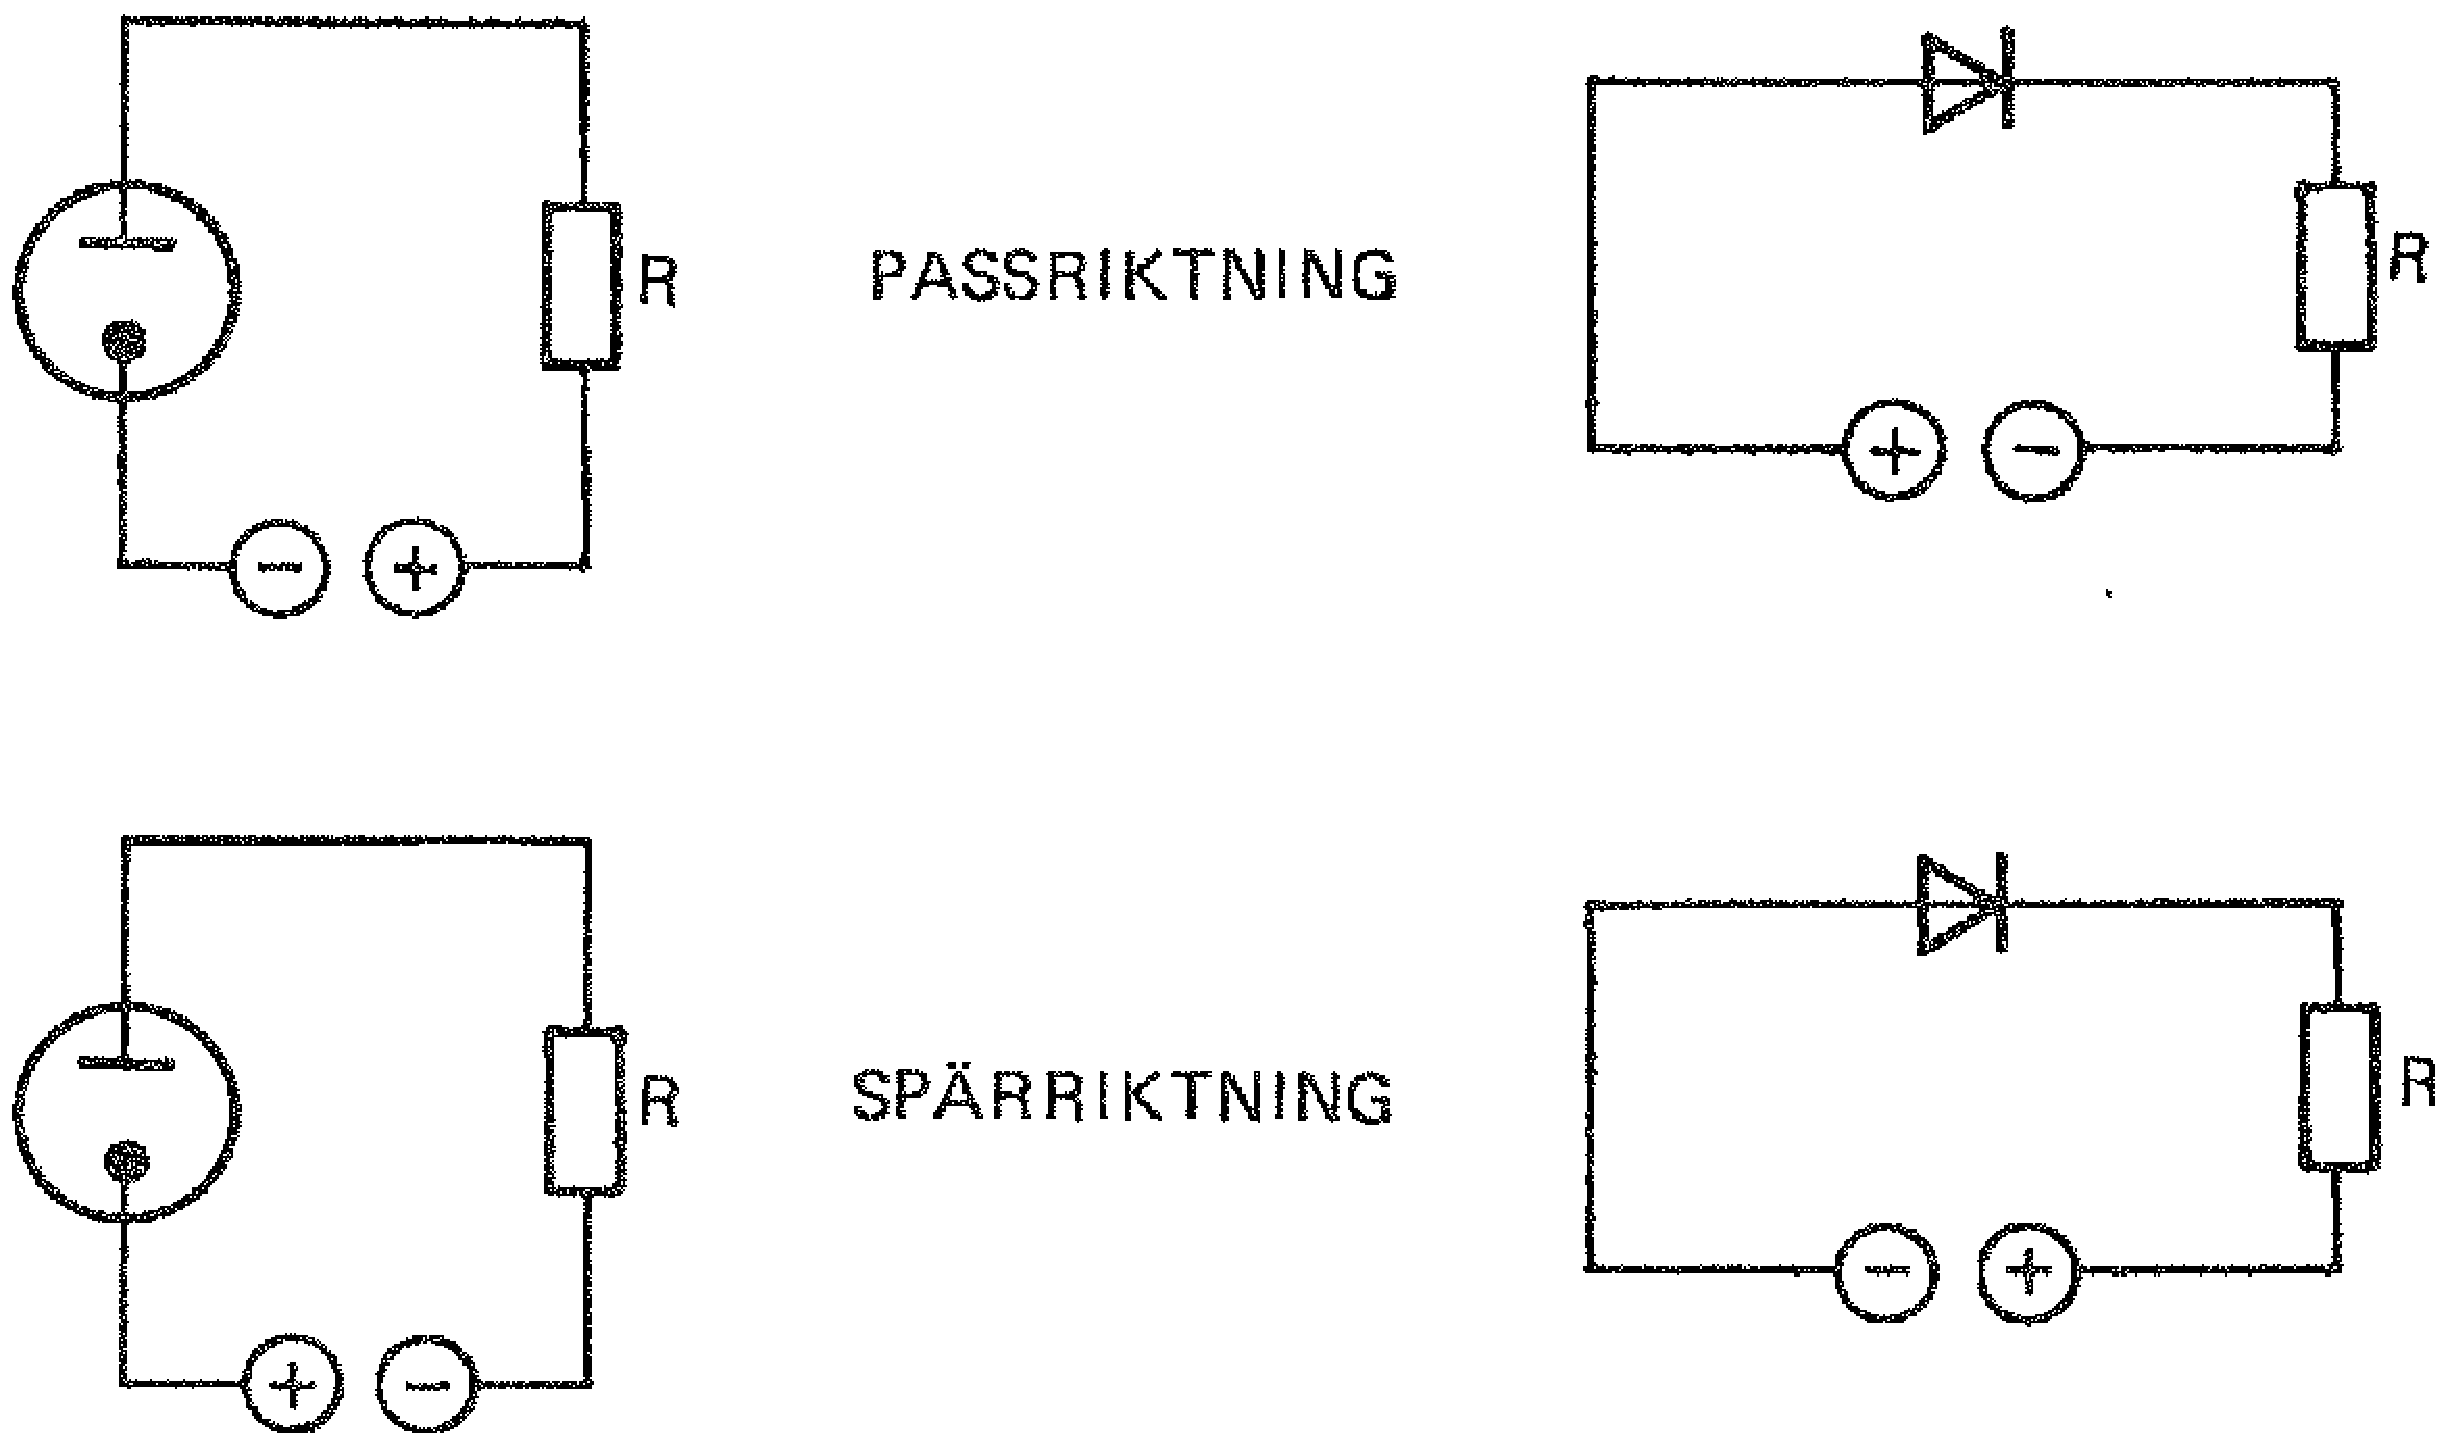
\includegraphics[width=\textwidth]{images/cropped_pdfs/bild_2_2-15.pdf}
\caption{Dioders polarisering i kretsen}
\label{fig:BildII2-15}
\end{figure}

Bild \ref{fig:BildII2-15} visar principen för hur de båda diodtyperna ingår i
en strömkrets.
Den stora skillnaden är att arbetsspänningen för en vakuumdiod är mångfalt
högre än den för en halvledardiod samt att vakuumdiodens ena elektrod (katoden)
behöver hettas upp för att avge elektroner.
